% Options for packages loaded elsewhere
\PassOptionsToPackage{unicode}{hyperref}
\PassOptionsToPackage{hyphens}{url}
%
\documentclass[
]{article}
\usepackage{lmodern}
\usepackage{amssymb,amsmath}
\usepackage{ifxetex,ifluatex}
\ifnum 0\ifxetex 1\fi\ifluatex 1\fi=0 % if pdftex
  \usepackage[T1]{fontenc}
  \usepackage[utf8]{inputenc}
  \usepackage{textcomp} % provide euro and other symbols
\else % if luatex or xetex
  \usepackage{unicode-math}
  \defaultfontfeatures{Scale=MatchLowercase}
  \defaultfontfeatures[\rmfamily]{Ligatures=TeX,Scale=1}
\fi
% Use upquote if available, for straight quotes in verbatim environments
\IfFileExists{upquote.sty}{\usepackage{upquote}}{}
\IfFileExists{microtype.sty}{% use microtype if available
  \usepackage[]{microtype}
  \UseMicrotypeSet[protrusion]{basicmath} % disable protrusion for tt fonts
}{}
\makeatletter
\@ifundefined{KOMAClassName}{% if non-KOMA class
  \IfFileExists{parskip.sty}{%
    \usepackage{parskip}
  }{% else
    \setlength{\parindent}{0pt}
    \setlength{\parskip}{6pt plus 2pt minus 1pt}}
}{% if KOMA class
  \KOMAoptions{parskip=half}}
\makeatother
\usepackage{xcolor}
\IfFileExists{xurl.sty}{\usepackage{xurl}}{} % add URL line breaks if available
\IfFileExists{bookmark.sty}{\usepackage{bookmark}}{\usepackage{hyperref}}
\hypersetup{
  pdftitle={Econometrics II - Problem 7},
  pdfauthor={William Radaic Peron},
  hidelinks,
  pdfcreator={LaTeX via pandoc}}
\urlstyle{same} % disable monospaced font for URLs
\usepackage[margin=1in]{geometry}
\usepackage{color}
\usepackage{fancyvrb}
\newcommand{\VerbBar}{|}
\newcommand{\VERB}{\Verb[commandchars=\\\{\}]}
\DefineVerbatimEnvironment{Highlighting}{Verbatim}{commandchars=\\\{\}}
% Add ',fontsize=\small' for more characters per line
\usepackage{framed}
\definecolor{shadecolor}{RGB}{248,248,248}
\newenvironment{Shaded}{\begin{snugshade}}{\end{snugshade}}
\newcommand{\AlertTok}[1]{\textcolor[rgb]{0.94,0.16,0.16}{#1}}
\newcommand{\AnnotationTok}[1]{\textcolor[rgb]{0.56,0.35,0.01}{\textbf{\textit{#1}}}}
\newcommand{\AttributeTok}[1]{\textcolor[rgb]{0.77,0.63,0.00}{#1}}
\newcommand{\BaseNTok}[1]{\textcolor[rgb]{0.00,0.00,0.81}{#1}}
\newcommand{\BuiltInTok}[1]{#1}
\newcommand{\CharTok}[1]{\textcolor[rgb]{0.31,0.60,0.02}{#1}}
\newcommand{\CommentTok}[1]{\textcolor[rgb]{0.56,0.35,0.01}{\textit{#1}}}
\newcommand{\CommentVarTok}[1]{\textcolor[rgb]{0.56,0.35,0.01}{\textbf{\textit{#1}}}}
\newcommand{\ConstantTok}[1]{\textcolor[rgb]{0.00,0.00,0.00}{#1}}
\newcommand{\ControlFlowTok}[1]{\textcolor[rgb]{0.13,0.29,0.53}{\textbf{#1}}}
\newcommand{\DataTypeTok}[1]{\textcolor[rgb]{0.13,0.29,0.53}{#1}}
\newcommand{\DecValTok}[1]{\textcolor[rgb]{0.00,0.00,0.81}{#1}}
\newcommand{\DocumentationTok}[1]{\textcolor[rgb]{0.56,0.35,0.01}{\textbf{\textit{#1}}}}
\newcommand{\ErrorTok}[1]{\textcolor[rgb]{0.64,0.00,0.00}{\textbf{#1}}}
\newcommand{\ExtensionTok}[1]{#1}
\newcommand{\FloatTok}[1]{\textcolor[rgb]{0.00,0.00,0.81}{#1}}
\newcommand{\FunctionTok}[1]{\textcolor[rgb]{0.00,0.00,0.00}{#1}}
\newcommand{\ImportTok}[1]{#1}
\newcommand{\InformationTok}[1]{\textcolor[rgb]{0.56,0.35,0.01}{\textbf{\textit{#1}}}}
\newcommand{\KeywordTok}[1]{\textcolor[rgb]{0.13,0.29,0.53}{\textbf{#1}}}
\newcommand{\NormalTok}[1]{#1}
\newcommand{\OperatorTok}[1]{\textcolor[rgb]{0.81,0.36,0.00}{\textbf{#1}}}
\newcommand{\OtherTok}[1]{\textcolor[rgb]{0.56,0.35,0.01}{#1}}
\newcommand{\PreprocessorTok}[1]{\textcolor[rgb]{0.56,0.35,0.01}{\textit{#1}}}
\newcommand{\RegionMarkerTok}[1]{#1}
\newcommand{\SpecialCharTok}[1]{\textcolor[rgb]{0.00,0.00,0.00}{#1}}
\newcommand{\SpecialStringTok}[1]{\textcolor[rgb]{0.31,0.60,0.02}{#1}}
\newcommand{\StringTok}[1]{\textcolor[rgb]{0.31,0.60,0.02}{#1}}
\newcommand{\VariableTok}[1]{\textcolor[rgb]{0.00,0.00,0.00}{#1}}
\newcommand{\VerbatimStringTok}[1]{\textcolor[rgb]{0.31,0.60,0.02}{#1}}
\newcommand{\WarningTok}[1]{\textcolor[rgb]{0.56,0.35,0.01}{\textbf{\textit{#1}}}}
\usepackage{graphicx,grffile}
\makeatletter
\def\maxwidth{\ifdim\Gin@nat@width>\linewidth\linewidth\else\Gin@nat@width\fi}
\def\maxheight{\ifdim\Gin@nat@height>\textheight\textheight\else\Gin@nat@height\fi}
\makeatother
% Scale images if necessary, so that they will not overflow the page
% margins by default, and it is still possible to overwrite the defaults
% using explicit options in \includegraphics[width, height, ...]{}
\setkeys{Gin}{width=\maxwidth,height=\maxheight,keepaspectratio}
% Set default figure placement to htbp
\makeatletter
\def\fps@figure{htbp}
\makeatother
\setlength{\emergencystretch}{3em} % prevent overfull lines
\providecommand{\tightlist}{%
  \setlength{\itemsep}{0pt}\setlength{\parskip}{0pt}}
\setcounter{secnumdepth}{-\maxdimen} % remove section numbering

\title{Econometrics II - Problem 7}
\author{William Radaic Peron}
\date{\today}

\begin{document}
\maketitle

\begin{Shaded}
\begin{Highlighting}[]
\KeywordTok{library}\NormalTok{(readxl)}
\KeywordTok{library}\NormalTok{(ggplot2)}
\KeywordTok{library}\NormalTok{(forecast)}
\KeywordTok{library}\NormalTok{(dynlm)}
\KeywordTok{library}\NormalTok{(ggthemes)}
\KeywordTok{library}\NormalTok{(strucchange)}
\end{Highlighting}
\end{Shaded}

\begin{verbatim}
## 
## Attaching package: 'strucchange'
\end{verbatim}

\begin{verbatim}
## The following object is masked from 'package:stringr':
## 
##     boundary
\end{verbatim}

\begin{Shaded}
\begin{Highlighting}[]
\KeywordTok{library}\NormalTok{(lmtest)}
\KeywordTok{library}\NormalTok{(car)}
\KeywordTok{library}\NormalTok{(dplyr)}

\NormalTok{df <-}\StringTok{ }\KeywordTok{read_excel}\NormalTok{(}\StringTok{"G:/My Drive/FGV EESP/4o SEMESTRE/Econometria II/QuantEconEESP/QuantEconEESP/pibeua_real.xlsx"}\NormalTok{)}
\end{Highlighting}
\end{Shaded}

\begin{verbatim}
## New names:
## * `` -> ...1
\end{verbatim}

\begin{Shaded}
\begin{Highlighting}[]
\NormalTok{series <-}\StringTok{ }\KeywordTok{ts}\NormalTok{(df}\OperatorTok{$}\StringTok{`}\DataTypeTok{Cresimento percentual}\StringTok{`}\NormalTok{[}\DecValTok{13}\OperatorTok{:}\DecValTok{236}\NormalTok{], }\DataTypeTok{start =} \KeywordTok{c}\NormalTok{(}\DecValTok{1950}\NormalTok{, }
    \DecValTok{1}\NormalTok{), }\DataTypeTok{end =} \KeywordTok{c}\NormalTok{(}\DecValTok{2005}\NormalTok{, }\DecValTok{4}\NormalTok{), }\DataTypeTok{frequency =} \DecValTok{4}\NormalTok{)  }\CommentTok{# 1950-2005}

\KeywordTok{autoplot}\NormalTok{(series) }\OperatorTok{+}\StringTok{ }\KeywordTok{theme_few}\NormalTok{() }\OperatorTok{+}\StringTok{ }\KeywordTok{ggtitle}\NormalTok{(}\StringTok{"US GDP, 1950-2005"}\NormalTok{)}
\end{Highlighting}
\end{Shaded}

\begin{center}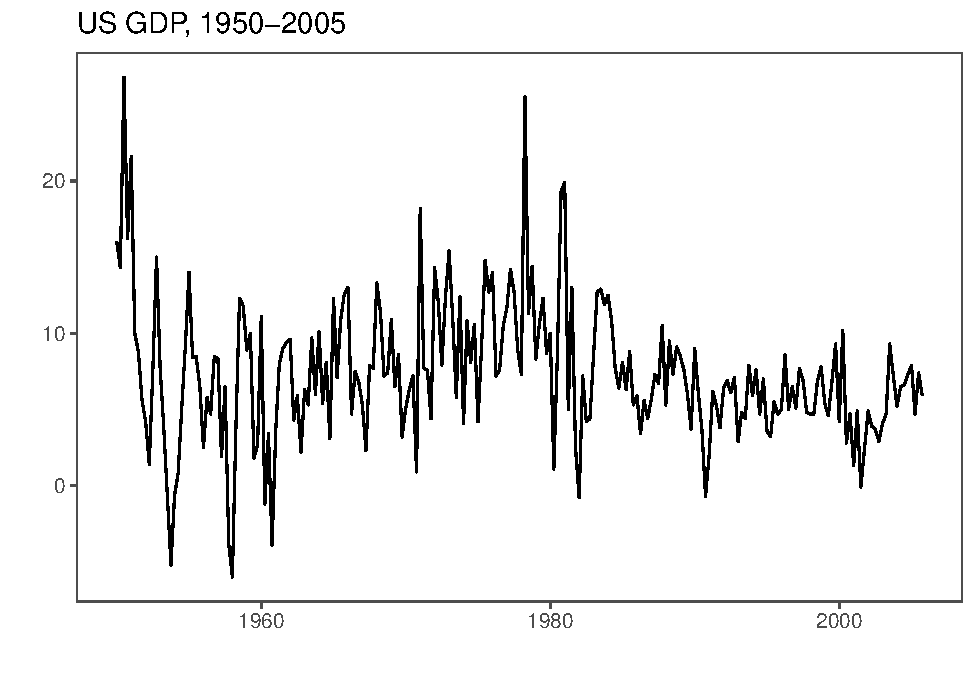
\includegraphics{Econo2_P7_files/figure-latex/all-1} \end{center}

\begin{Shaded}
\begin{Highlighting}[]
\CommentTok{# We can clearly see a reduction in variance during the 80s.}

\NormalTok{df}\OperatorTok{$}\NormalTok{observ <-}\StringTok{ }\DecValTok{1}\OperatorTok{:}\KeywordTok{length}\NormalTok{(df}\OperatorTok{$}\StringTok{`}\DataTypeTok{PIB nominal}\StringTok{`}\NormalTok{)}

\CommentTok{# Suppose that the break happens at time t = 153 (Q1, 1985).}

\NormalTok{df}\OperatorTok{$}\NormalTok{d <-}\StringTok{ }\KeywordTok{as.numeric}\NormalTok{(df}\OperatorTok{$}\NormalTok{observ }\OperatorTok{>}\StringTok{ }\DecValTok{152}\NormalTok{)}

\NormalTok{m1 <-}\StringTok{ }\KeywordTok{lm}\NormalTok{(series }\OperatorTok{~}\StringTok{ }\NormalTok{df}\OperatorTok{$}\NormalTok{d[}\DecValTok{13}\OperatorTok{:}\DecValTok{236}\NormalTok{])}

\KeywordTok{summary}\NormalTok{(m1)}
\end{Highlighting}
\end{Shaded}

\begin{verbatim}
## 
## Call:
## lm(formula = series ~ df$d[13:236])
## 
## Residuals:
##      Min       1Q   Median       3Q      Max 
## -14.2379  -2.0571  -0.1379   2.2871  18.5621 
## 
## Coefficients:
##              Estimate Std. Error t value Pr(>|t|)    
## (Intercept)    8.2379     0.3728  22.098  < 2e-16 ***
## df$d[13:236]  -2.5057     0.6088  -4.116 5.43e-05 ***
## ---
## Signif. codes:  0 '***' 0.001 '**' 0.01 '*' 0.05 '.' 0.1 ' ' 1
## 
## Residual standard error: 4.411 on 222 degrees of freedom
## Multiple R-squared:  0.0709, Adjusted R-squared:  0.06672 
## F-statistic: 16.94 on 1 and 222 DF,  p-value: 5.435e-05
\end{verbatim}

\begin{Shaded}
\begin{Highlighting}[]
\NormalTok{m2 <-}\StringTok{ }\KeywordTok{dynlm}\NormalTok{(series }\OperatorTok{~}\StringTok{ }\NormalTok{df}\OperatorTok{$}\NormalTok{d[}\DecValTok{13}\OperatorTok{:}\DecValTok{236}\NormalTok{] }\OperatorTok{+}\StringTok{ }\KeywordTok{L}\NormalTok{(series, }\DecValTok{1}\NormalTok{) }\OperatorTok{+}\StringTok{ }\KeywordTok{L}\NormalTok{(series, }
    \DecValTok{1}\NormalTok{) }\OperatorTok{*}\StringTok{ }\NormalTok{df}\OperatorTok{$}\NormalTok{d[}\DecValTok{13}\OperatorTok{:}\DecValTok{236}\NormalTok{])}

\KeywordTok{summary}\NormalTok{(m2)}
\end{Highlighting}
\end{Shaded}

\begin{verbatim}
## 
## Time series regression with "ts" data:
## Start = 1950(2), End = 2005(4)
## 
## Call:
## dynlm(formula = series ~ df$d[13:236] + L(series, 1) + L(series, 
##     1) * df$d[13:236])
## 
## Residuals:
##      Min       1Q   Median       3Q      Max 
## -11.2567  -2.1410  -0.0335   2.0335  17.7119 
## 
## Coefficients:
##                           Estimate Std. Error t value Pr(>|t|)    
## (Intercept)                4.76430    0.63168   7.542 1.22e-12 ***
## df$d[13:236]              -0.40507    1.40339  -0.289    0.773    
## L(series, 1)               0.41421    0.06436   6.436 7.63e-10 ***
## df$d[13:236]:L(series, 1) -0.17495    0.21438  -0.816    0.415    
## ---
## Signif. codes:  0 '***' 0.001 '**' 0.01 '*' 0.05 '.' 0.1 ' ' 1
## 
## Residual standard error: 4.033 on 219 degrees of freedom
## Multiple R-squared:  0.2209, Adjusted R-squared:  0.2103 
## F-statistic:  20.7 on 3 and 219 DF,  p-value: 7.576e-12
\end{verbatim}

\begin{Shaded}
\begin{Highlighting}[]
\CommentTok{# ARIMA model}

\NormalTok{arima_unr <-}\StringTok{ }\KeywordTok{arima}\NormalTok{(series, }\DataTypeTok{order =} \KeywordTok{c}\NormalTok{(}\DecValTok{1}\NormalTok{, }\DecValTok{0}\NormalTok{, }\DecValTok{0}\NormalTok{))}

\NormalTok{arima_r1 <-}\StringTok{ }\KeywordTok{arima}\NormalTok{(series[}\DecValTok{1}\OperatorTok{:}\DecValTok{152}\NormalTok{], }\DataTypeTok{order =} \KeywordTok{c}\NormalTok{(}\DecValTok{1}\NormalTok{, }\DecValTok{0}\NormalTok{, }\DecValTok{0}\NormalTok{))}

\NormalTok{arima_r2 <-}\StringTok{ }\KeywordTok{arima}\NormalTok{(series[}\DecValTok{153}\OperatorTok{:}\KeywordTok{length}\NormalTok{(series)], }\DataTypeTok{order =} \KeywordTok{c}\NormalTok{(}\DecValTok{1}\NormalTok{, }\DecValTok{0}\NormalTok{, }
    \DecValTok{0}\NormalTok{))}

\NormalTok{ssr_unr <-}\StringTok{ }\KeywordTok{sum}\NormalTok{(arima_unr}\OperatorTok{$}\NormalTok{residuals}\OperatorTok{^}\DecValTok{2}\NormalTok{)}

\NormalTok{ssr_r1 <-}\StringTok{ }\KeywordTok{sum}\NormalTok{(arima_r1}\OperatorTok{$}\NormalTok{residuals}\OperatorTok{^}\DecValTok{2}\NormalTok{)}

\NormalTok{ssr_r2 <-}\StringTok{ }\KeywordTok{sum}\NormalTok{(arima_r2}\OperatorTok{$}\NormalTok{residuals}\OperatorTok{^}\DecValTok{2}\NormalTok{)}

\CommentTok{# We will now define the Chow test for the null H0: \textbackslash{}beta_m1}
\CommentTok{# - \textbackslash{}beta_m2 = 0 (no structural break)}

\NormalTok{chow <-}\StringTok{ }\ControlFlowTok{function}\NormalTok{(SSR_unr, SSR_r1, SSR_r2, t, n) \{}
    
\NormalTok{    ((SSR_unr }\OperatorTok{-}\StringTok{ }\NormalTok{SSR_r1 }\OperatorTok{-}\StringTok{ }\NormalTok{SSR_r2)}\OperatorTok{/}\NormalTok{n)}\OperatorTok{/}\NormalTok{((SSR_r1 }\OperatorTok{+}\StringTok{ }\NormalTok{SSR_r2)}\OperatorTok{/}\NormalTok{(t }\OperatorTok{-}\StringTok{ }\DecValTok{2} \OperatorTok{*}\StringTok{ }
\StringTok{        }\NormalTok{n))}
    
\NormalTok{\}}


\KeywordTok{chow}\NormalTok{(}\DataTypeTok{SSR_unr =}\NormalTok{ ssr_unr, }\DataTypeTok{SSR_r1 =}\NormalTok{ ssr_r1, }\DataTypeTok{SSR_r2 =}\NormalTok{ ssr_r2, }\DataTypeTok{t =} \KeywordTok{length}\NormalTok{(series), }
    \DataTypeTok{n =} \KeywordTok{length}\NormalTok{(arima_unr}\OperatorTok{$}\NormalTok{coef))  }\CommentTok{# T statistic (n, T - 2n).}
\end{Highlighting}
\end{Shaded}

\begin{verbatim}
## [1] 3.736208
\end{verbatim}

\begin{Shaded}
\begin{Highlighting}[]
\CommentTok{# Now, suppose that we do not know when the break happened.}

\NormalTok{t0 =}\StringTok{ }\DecValTok{45}
\NormalTok{tf =}\StringTok{ }\DecValTok{180}  \CommentTok{# Boundaries for the process.}

\NormalTok{models =}\StringTok{ }\KeywordTok{list}\NormalTok{(}\OtherTok{NA}\NormalTok{)}

\NormalTok{coefs =}\StringTok{ }\KeywordTok{matrix}\NormalTok{(}\OtherTok{NA}\NormalTok{, }\DataTypeTok{nrow =} \KeywordTok{length}\NormalTok{(t0}\OperatorTok{:}\NormalTok{tf), }\DataTypeTok{ncol =} \DecValTok{2}\NormalTok{)}

\NormalTok{forecasts =}\StringTok{ }\KeywordTok{list}\NormalTok{(}\OtherTok{NA}\NormalTok{)}

\NormalTok{ci =}\StringTok{ }\KeywordTok{data.frame}\NormalTok{(}\KeywordTok{matrix}\NormalTok{(}\OtherTok{NA}\NormalTok{, }\DataTypeTok{nrow =} \KeywordTok{length}\NormalTok{(t0}\OperatorTok{:}\NormalTok{tf), }\DataTypeTok{ncol =} \DecValTok{5}\NormalTok{))}

\NormalTok{e =}\StringTok{ }\KeywordTok{matrix}\NormalTok{(}\OtherTok{NA}\NormalTok{, }\DataTypeTok{nrow =} \KeywordTok{length}\NormalTok{(t0}\OperatorTok{:}\NormalTok{tf), }\DataTypeTok{ncol =} \DecValTok{1}\NormalTok{)}


\CommentTok{# 1. Plotting coefficients.}

\ControlFlowTok{for}\NormalTok{ (i }\ControlFlowTok{in}\NormalTok{ (}\DecValTok{1}\OperatorTok{:}\NormalTok{(tf }\OperatorTok{-}\StringTok{ }\NormalTok{t0))) \{}
    
\NormalTok{    models[[i]] =}\StringTok{ }\KeywordTok{arima}\NormalTok{(series[}\DecValTok{1}\OperatorTok{:}\NormalTok{(i }\OperatorTok{+}\StringTok{ }\NormalTok{t0)], }\DataTypeTok{order =} \KeywordTok{c}\NormalTok{(}\DecValTok{1}\NormalTok{, }\DecValTok{0}\NormalTok{, }\DecValTok{0}\NormalTok{))}
    
\NormalTok{    coefs[i, ] =}\StringTok{ }\NormalTok{models[[i]]}\OperatorTok{$}\NormalTok{coef}
    
\NormalTok{    forecasts[[i]] =}\StringTok{ }\KeywordTok{forecast}\NormalTok{(series[}\DecValTok{1}\OperatorTok{:}\NormalTok{(i }\OperatorTok{+}\StringTok{ }\NormalTok{t0)], }\DataTypeTok{model =}\NormalTok{ models[[i]], }
        \DataTypeTok{h =} \DecValTok{1}\NormalTok{)}
    
\NormalTok{    e[i, ] =}\StringTok{ }\NormalTok{forecasts[[i]]}\OperatorTok{$}\NormalTok{mean }\OperatorTok{-}\StringTok{ }\NormalTok{series[(i }\OperatorTok{+}\StringTok{ }\NormalTok{t0 }\OperatorTok{+}\StringTok{ }\DecValTok{1}\NormalTok{)]}
    
\NormalTok{\}}

\NormalTok{coefs =}\StringTok{ }\KeywordTok{data.frame}\NormalTok{(coefs)}

\NormalTok{coefs =}\StringTok{ }\KeywordTok{data.frame}\NormalTok{(coefs, (}\DecValTok{1}\OperatorTok{:}\KeywordTok{length}\NormalTok{(coefs}\OperatorTok{$}\NormalTok{X1)))}

\NormalTok{df.coefs =}\StringTok{ }\KeywordTok{na.omit}\NormalTok{(}\KeywordTok{data.frame}\NormalTok{(coefs))}

\KeywordTok{names}\NormalTok{(df.coefs) =}\StringTok{ }\KeywordTok{c}\NormalTok{(}\StringTok{"ar1"}\NormalTok{, }\StringTok{"intercept"}\NormalTok{, }\StringTok{"index"}\NormalTok{)}

\KeywordTok{ggplot}\NormalTok{(df.coefs, }\KeywordTok{aes}\NormalTok{(}\DataTypeTok{x =}\NormalTok{ index, }\DataTypeTok{y =}\NormalTok{ ar1)) }\OperatorTok{+}\StringTok{ }\KeywordTok{geom_line}\NormalTok{() }\OperatorTok{+}\StringTok{ }\KeywordTok{theme_few}\NormalTok{()}
\end{Highlighting}
\end{Shaded}

\begin{center}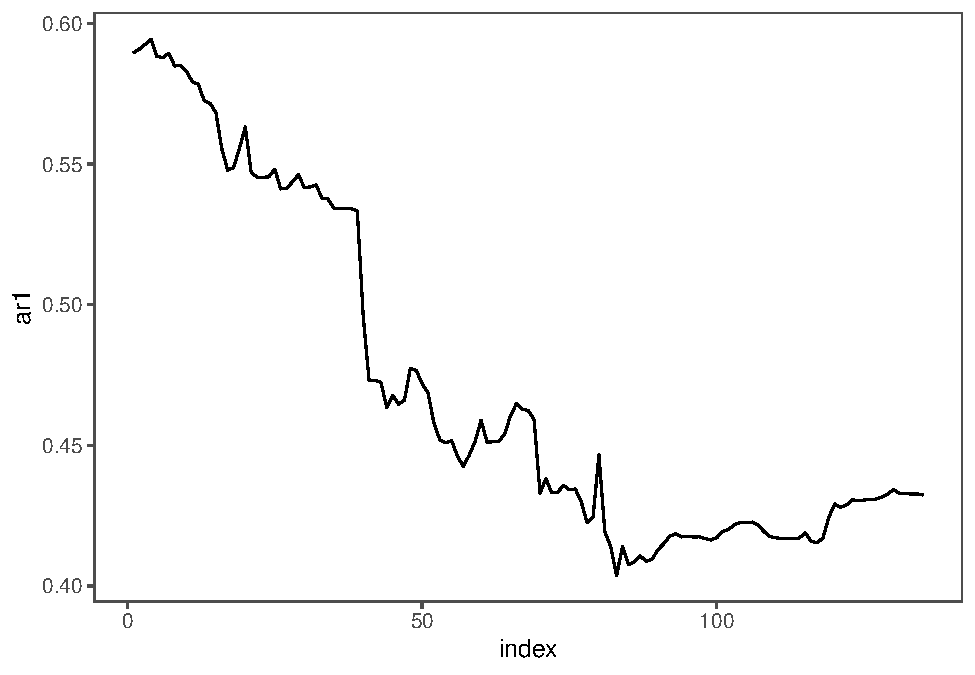
\includegraphics{Econo2_P7_files/figure-latex/all-2} \end{center}

\begin{Shaded}
\begin{Highlighting}[]
\KeywordTok{ggplot}\NormalTok{(df.coefs, }\KeywordTok{aes}\NormalTok{(}\DataTypeTok{x =}\NormalTok{ index, }\DataTypeTok{y =}\NormalTok{ intercept)) }\OperatorTok{+}\StringTok{ }\KeywordTok{geom_line}\NormalTok{() }\OperatorTok{+}\StringTok{ }
\StringTok{    }\KeywordTok{theme_few}\NormalTok{()}
\end{Highlighting}
\end{Shaded}

\begin{center}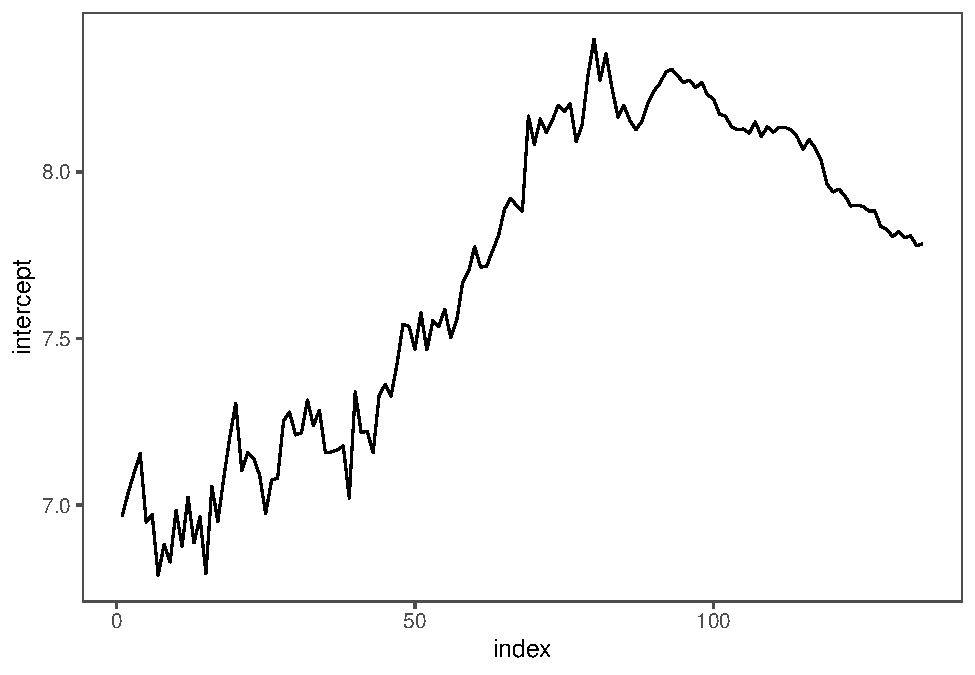
\includegraphics{Econo2_P7_files/figure-latex/all-3} \end{center}

\begin{Shaded}
\begin{Highlighting}[]
\CommentTok{# 2. Cusum test.}

\NormalTok{cusums =}\StringTok{ }\KeywordTok{matrix}\NormalTok{(}\OtherTok{NA}\NormalTok{, }\DataTypeTok{nrow =} \KeywordTok{length}\NormalTok{(e), }\DataTypeTok{ncol =} \DecValTok{1}\NormalTok{)}

\NormalTok{e =}\StringTok{ }\KeywordTok{na.omit}\NormalTok{(e)}

\ControlFlowTok{for}\NormalTok{ (i }\ControlFlowTok{in} \DecValTok{1}\OperatorTok{:}\NormalTok{(}\KeywordTok{length}\NormalTok{(e))) \{}
    
\NormalTok{    cusums[i, ] =}\StringTok{ }\KeywordTok{sum}\NormalTok{(e[}\DecValTok{1}\OperatorTok{:}\NormalTok{i])}\OperatorTok{/}\KeywordTok{sd}\NormalTok{(e)}
    
\NormalTok{\}}


\NormalTok{cusums =}\StringTok{ }\KeywordTok{na.omit}\NormalTok{(cusums)}

\NormalTok{df.cusums =}\StringTok{ }\KeywordTok{data.frame}\NormalTok{(cusums)}

\KeywordTok{ggplot}\NormalTok{(df.cusums, }\KeywordTok{aes}\NormalTok{(}\DataTypeTok{x =}\NormalTok{ (}\DecValTok{1}\OperatorTok{:}\KeywordTok{length}\NormalTok{(cusums)), }\DataTypeTok{y =}\NormalTok{ cusums)) }\OperatorTok{+}\StringTok{ }
\StringTok{    }\KeywordTok{geom_line}\NormalTok{() }\OperatorTok{+}\StringTok{ }\KeywordTok{theme_few}\NormalTok{()}
\end{Highlighting}
\end{Shaded}

\begin{center}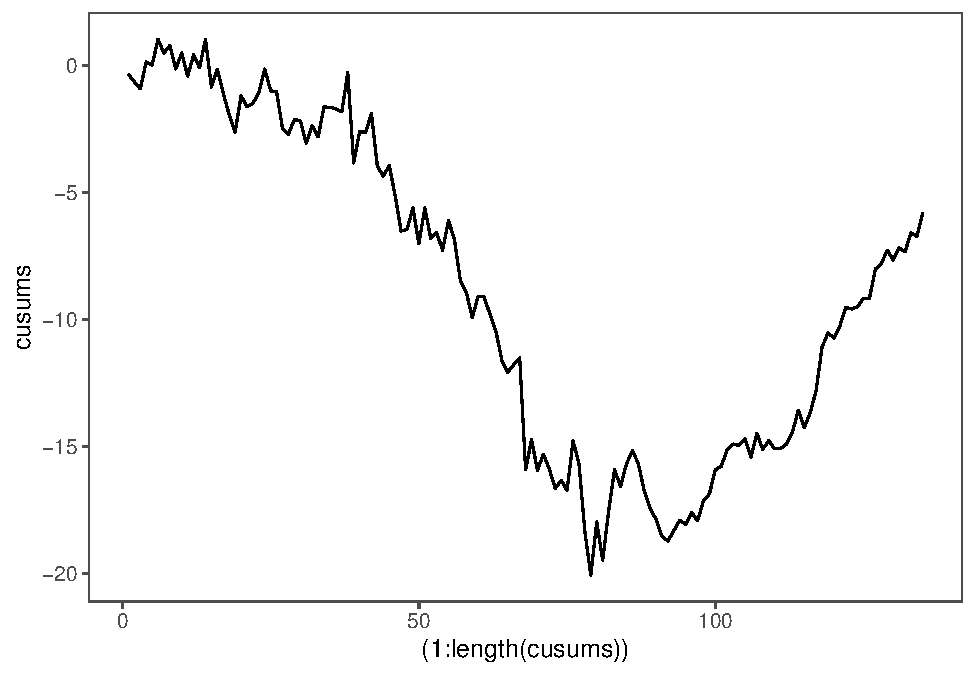
\includegraphics{Econo2_P7_files/figure-latex/all-4} \end{center}

\begin{Shaded}
\begin{Highlighting}[]
\CommentTok{# 3. Iterative F-tests.}

\NormalTok{models_unr =}\StringTok{ }\KeywordTok{list}\NormalTok{(}\OtherTok{NA}\NormalTok{)}

\NormalTok{models_r =}\StringTok{ }\KeywordTok{list}\NormalTok{(}\OtherTok{NA}\NormalTok{)}


\CommentTok{# dummy <- df$d[13:236]}

\NormalTok{num_series =}\StringTok{ }\KeywordTok{as.numeric}\NormalTok{(series)}

\NormalTok{f_values =}\StringTok{ }\KeywordTok{matrix}\NormalTok{(}\OtherTok{NA}\NormalTok{, }\DataTypeTok{nrow =} \KeywordTok{length}\NormalTok{(num_series), }\DataTypeTok{ncol =} \DecValTok{2}\NormalTok{)}

\NormalTok{hyp =}\StringTok{ }\KeywordTok{c}\NormalTok{(}\DecValTok{0}\NormalTok{, }\DecValTok{-1}\NormalTok{, }\DecValTok{0}\NormalTok{, }\DecValTok{1}\NormalTok{)}

\NormalTok{rhs =}\StringTok{ }\DecValTok{0}

\KeywordTok{length}\NormalTok{((t0}\OperatorTok{:}\NormalTok{tf))}
\end{Highlighting}
\end{Shaded}

\begin{verbatim}
## [1] 136
\end{verbatim}

\begin{Shaded}
\begin{Highlighting}[]
\NormalTok{dummies =}\StringTok{ }\KeywordTok{data.frame}\NormalTok{(}\KeywordTok{matrix}\NormalTok{(}\OtherTok{NA}\NormalTok{, }\DataTypeTok{ncol =} \DecValTok{224}\NormalTok{, }\DataTypeTok{nrow =} \DecValTok{224}\NormalTok{))}

\ControlFlowTok{for}\NormalTok{ (i }\ControlFlowTok{in}\NormalTok{ (}\DecValTok{13}\OperatorTok{:}\DecValTok{236}\NormalTok{)) \{}
\NormalTok{    dummies[i] =}\StringTok{ }\KeywordTok{as.numeric}\NormalTok{(df}\OperatorTok{$}\NormalTok{observ[}\DecValTok{13}\OperatorTok{:}\DecValTok{236}\NormalTok{] }\OperatorTok{>=}\StringTok{ }\NormalTok{i)}
\NormalTok{\}}


\ControlFlowTok{for}\NormalTok{ (i }\ControlFlowTok{in}\NormalTok{ (}\DecValTok{1}\OperatorTok{:}\NormalTok{(tf }\OperatorTok{-}\StringTok{ }\NormalTok{t0))) \{}
    
\NormalTok{    adummy <-}\StringTok{ }\KeywordTok{rep}\NormalTok{(}\DecValTok{0}\NormalTok{, }\DecValTok{1}\NormalTok{)}
\NormalTok{    j <-}\StringTok{ }\DecValTok{0}
\NormalTok{    k <-}\StringTok{ }\NormalTok{t0 }\OperatorTok{+}\StringTok{ }\NormalTok{i}
    \ControlFlowTok{while}\NormalTok{ (j }\OperatorTok{<=}\StringTok{ }\KeywordTok{length}\NormalTok{(num_series)) \{}
        \ControlFlowTok{if}\NormalTok{ (j }\OperatorTok{>}\StringTok{ }\NormalTok{k) \{}
            \CommentTok{# não sei se isso deveria ser maior ou igual ou só maior}
\NormalTok{            adummy[j] <-}\StringTok{ }\DecValTok{1}
\NormalTok{        \} }\ControlFlowTok{else}\NormalTok{ \{}
\NormalTok{            adummy[j] <-}\StringTok{ }\DecValTok{0}
\NormalTok{        \}}
\NormalTok{        j <-}\StringTok{ }\NormalTok{j }\OperatorTok{+}\StringTok{ }\DecValTok{1}
\NormalTok{    \}}
\NormalTok{    models_unr[[i]] <-}\StringTok{ }\KeywordTok{dynlm}\NormalTok{(num_series }\OperatorTok{~}\StringTok{ }\NormalTok{adummy }\OperatorTok{+}\StringTok{ }\KeywordTok{lag}\NormalTok{(num_series) }\OperatorTok{+}\StringTok{ }
\StringTok{        }\KeywordTok{lag}\NormalTok{(num_series) }\OperatorTok{*}\StringTok{ }\NormalTok{adummy)}
\NormalTok{    f_values[i, }\DecValTok{1}\NormalTok{] =}\StringTok{ }\KeywordTok{linearHypothesis}\NormalTok{(models_unr[[i]], hyp, rhs)}\OperatorTok{$}\NormalTok{F[}\DecValTok{1}\NormalTok{]}
\NormalTok{    f_values[i, }\DecValTok{2}\NormalTok{] =}\StringTok{ }\KeywordTok{linearHypothesis}\NormalTok{(models_unr[[i]], hyp, rhs)}\OperatorTok{$}\NormalTok{F[}\DecValTok{2}\NormalTok{]  }\CommentTok{#eu acho que funcionou?????}
    
\NormalTok{\}}

\NormalTok{df.f_values <-}\StringTok{ }\KeywordTok{data.frame}\NormalTok{(f_values)}

\NormalTok{df.f_values <-}\StringTok{ }\NormalTok{df.f_values}\OperatorTok{$}\NormalTok{X2}

\NormalTok{df.f_values <-}\StringTok{ }\KeywordTok{na.omit}\NormalTok{(df.f_values)}

\NormalTok{df.f_values <-}\StringTok{ }\KeywordTok{data.frame}\NormalTok{(df.f_values, ((t0 }\OperatorTok{+}\StringTok{ }\DecValTok{1}\NormalTok{)}\OperatorTok{:}\NormalTok{tf))}

\KeywordTok{names}\NormalTok{(df.f_values) <-}\StringTok{ }\KeywordTok{c}\NormalTok{(}\StringTok{"fvalue"}\NormalTok{, }\StringTok{"t"}\NormalTok{)}

\KeywordTok{ggplot}\NormalTok{(df.f_values, }\KeywordTok{aes}\NormalTok{(}\DataTypeTok{x =}\NormalTok{ t, }\DataTypeTok{y =}\NormalTok{ fvalue)) }\OperatorTok{+}\StringTok{ }\KeywordTok{geom_line}\NormalTok{() }\OperatorTok{+}\StringTok{ }\KeywordTok{theme_few}\NormalTok{()}
\end{Highlighting}
\end{Shaded}

\begin{center}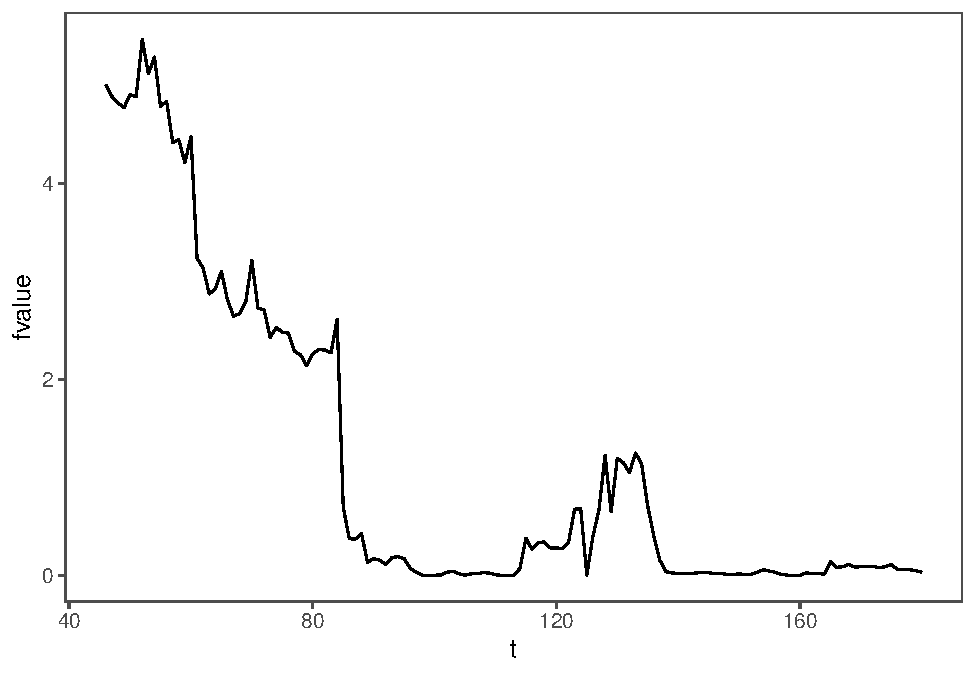
\includegraphics{Econo2_P7_files/figure-latex/all-5} \end{center}

\begin{Shaded}
\begin{Highlighting}[]
\KeywordTok{linearHypothesis}\NormalTok{(models_unr[[}\DecValTok{10}\NormalTok{]], hyp, rhs)}
\end{Highlighting}
\end{Shaded}

\begin{verbatim}
## Linear hypothesis test
## 
## Hypothesis:
## - adummy  + adummy:lag(num_series) = 0
## 
## Model 1: restricted model
## Model 2: num_series ~ adummy + lag(num_series) + lag(num_series) * adummy
## 
##   Res.Df    RSS Df Sum of Sq      F  Pr(>F)  
## 1    220 3673.8                              
## 2    219 3595.2  1    78.591 4.7874 0.02973 *
## ---
## Signif. codes:  0 '***' 0.001 '**' 0.01 '*' 0.05 '.' 0.1 ' ' 1
\end{verbatim}

\end{document}
